\chapter{Computer Applications}

In recent years, my approach to composing and performing music has reached a point were the development of computer applications runs simultaneously with my aesthetic and creative research. From the very start of composition and conception until the performance and realization, the computer applications that are developed and the artistic output merge within the same creative process. Therefore, my artistic practice is deeply connected to computer programming and the use of computer applications. It is worth mentioning that the applications developed as part of this process are vital to the musical results of the compositions and encompass an important aspect of the compositional process. In addition, these applications were developed for an artistic purpose and understanding how they work might give an insight into my compositional output. Moreover, they do not serve a function beyond the realization of the idiosyncratic elements that constitute my creative process. That is to say, these applications do not represent a contribution to the scientific community in relationship to the technological developments of computer music but instead represent a set of tools and documentation that other artists, musicians and composers might find useful for their own practice.

In the previous chapter, I explained some of the potential that technology has brought to music and how even though technological advancements do not necessarily represent artistic developments, they do provide with new possibilities for artistic innovation. It is because of these possibilities that I have become recently interested in using digital technology to create music. I am particularly interested in using technology for... 
 
In this chapter, I will explain in detail a number of important computer applications that were developed together with my compositional practice. These applications were written in the \href{http://supercollider.sourceforge.net/}{\mbox{SuperCollider}}\footnote{James McCartney, SuperCollider, 1996. URL: \href{http://www.audiosynth.com/}{http://www.audiosynth.com/}} programming language. I decided to use SuperCollider as a platform to develop these computer applications because it integrates a powerful audio synthesis server using state-of-the-art technology with the versatility and capabilities of an object-oriented-programming (OOP) language. I chose SuperCollider over other data flow programming applications like \href{http://www.cycling74.com/}{Max/MSP} and \href{http://puredata.info/}{Pure Data} (Pd) because of its robust synthesis server and the advantages of abstraction of a high-level OOP language.\footnote{See James McCartney, ``Rethinking the Computer Language: SuperCollider'', in \emph{Computer Music Journal}, volume 25, number 4, pp. 61-68, 2002, for a discussion about the differences between SuperCollider and Max/MSP, Pd and Csound.} Another advantage I saw in using SuperCollider is the fact that it is an open source application, which means that the code in which it is written is available for free and can be modified. Most of the computer applications I developed and which will be discussed in this chapter are written as SuperCollider classes,\footnote{SuperCollider classes are descriptions of the structure and implementation of a set of objects that represent the instances of the class.} but some of them are extensions of already existing classes or code that can be evaluated in real-time in the interpreter. The applications discussed in this chapter were used in various of the works submitted and constitute compositional strategies that reflect some aesthetic concerns that are recurrent in my work.

\section{Spectral Tracking}

In previous chapter, I briefly explained how spectralism and C. Barlow: \emph{Synthrumentation} influenced my work.

Fast Fourier Transform (FFT)\footnote{See Curtis Roads, \emph{The Computer Music Tutorial}, Cambridge, MA: MIT Press, 1996, pp. 533-609 for more information about spectrum analysis, including FFT.}


MIDI\footnote{See Ibid. pp. 969-1016 for more information about MIDI}

Spectrum analysis for dynamics, pitch and rhythm extraction. 


\subsection{PartialTracker}

\href{http://github.com/freuben/FedeLib/blob/master/PartialTracking/PartialTracker.sc}{PartialTracker} is a SuperCollider class for real-time partial extraction that diminishes the amount of FFT data by selecting the loudest bins and discarding the softer magnitudes with the purpose of having a limited amount of values to be returned as simple arrays for frequency and magnitude. It does so by taking an incoming audio signal, performing an FFT analysis and discarding spectral data in two ways: either by passing only the bins that are above a given magnitude threshold or by selecting a value that returns the strongest number of bins. For this purpose, I used the PV\_MagAbove and PV\_MaxMagN\footnote{PV\_MaxMagN is part of JoshUGens by \href{http://www.realizedsound.net/josh/}{Joshua Parmenter}, which is part of the \href{http://sourceforge.net/projects/sc3-plugins/}{sc3-plugins project}.} phase vocoder unit generators. In order to have access to this data in the language side of SuperCollider, I used PV\_MagBuffer and PV\_FreqBuffer\footnote{PV\_MagBuffer and PV\_FreqBuffer are part of JoshUGens.} to store this information into a buffer. Ones stored in a buffer, the information can be accessed as an array and be manipulated freely. Nevertheless, the buffer stores all of the bins of the FFT and therefore the bins with the magnitudes that were not empty have still to be collected and indexed to access the corresponding frequency values. The resulting arrays therefore only constitute the number of strongest bins, which can be defined by the user. The following code shows an example of the frequency and magnitude arrays for the ten strongest bins:

\begin{verbatim}
[ 128.37791442871, 154.57292175293, 140.25003051758, 246.26268005371, 253.09353637695,
 364.92492675781, 396.52267456055, 1035.068359375, 1037.1043701172, 1241.3063964844 ]; 
 //array of frequencies

[ 1.8754153251648, 4.5471153259277, 5.3137745857239, 2.6146886348724, 1.2295168638229,
  2.5435922145844, 3.215939283371, 2.0944044589996, 2.6014709472656, 2.0559096336365 ]; 
 //array of magnitudes
\end{verbatim}
The purpose of this class is to have easy access to relevant FFT information with the aim to convert frequencies and magnitudes either as MIDI messages or as data to be used to control synthesis definitions\footnote{Synthesis definitions, or SynthDefs in SuperCollider represent a description of a set of Unit Generators (UGens) that perform synthesis algorithms in the SuperCollider server.}. The incoming signal can be a live input in a performance situation, or a sound file. Lastly, this class also provides the feature of saving the spectral information trigged by an onset detector with the objective of  creating a MIDI file by storing time values and converting the frequency and magnitude data to MIDI notes and velocities.

\subsection{FFTFilter}

\href{http://github.com/freuben/FedeLib/blob/master/PartialTracking/PartialTracker.sc}{FFTFilter} inherits functionality from PartialTracker and uses the information of the frequency array to control the bandwidth and center frequency of a two pole resonant filter. This FFT controlled filter is designed to be used to filter a signal with a rich spectral content, such as different types of noise, with the information given by an FFT analysis of another signal that should be more limited in its frequency range. A function is evaluated in a loop in which an argument that can be changed by the user represents the time value between each iteration. This function accesses the highest and lowest frequency values from the array calculated by the PartialTracker functionality every time the loop is evaluated. Since the purpose is to make a smooth line instead of discrete points, the signal must be lagged exponentially to produce a continuous control signal. By following this procedure, it is possible to approximately track the contour of the frequencies that have a stronger presence, given that the settings for the amount of strongest bins and magnitude threshold are appropriate for the specific spectral characteristics of the signal. Figure 4.1 
\begin{figure}[htbp] %  figure placement: here, top, bottom, or page
   \centering
   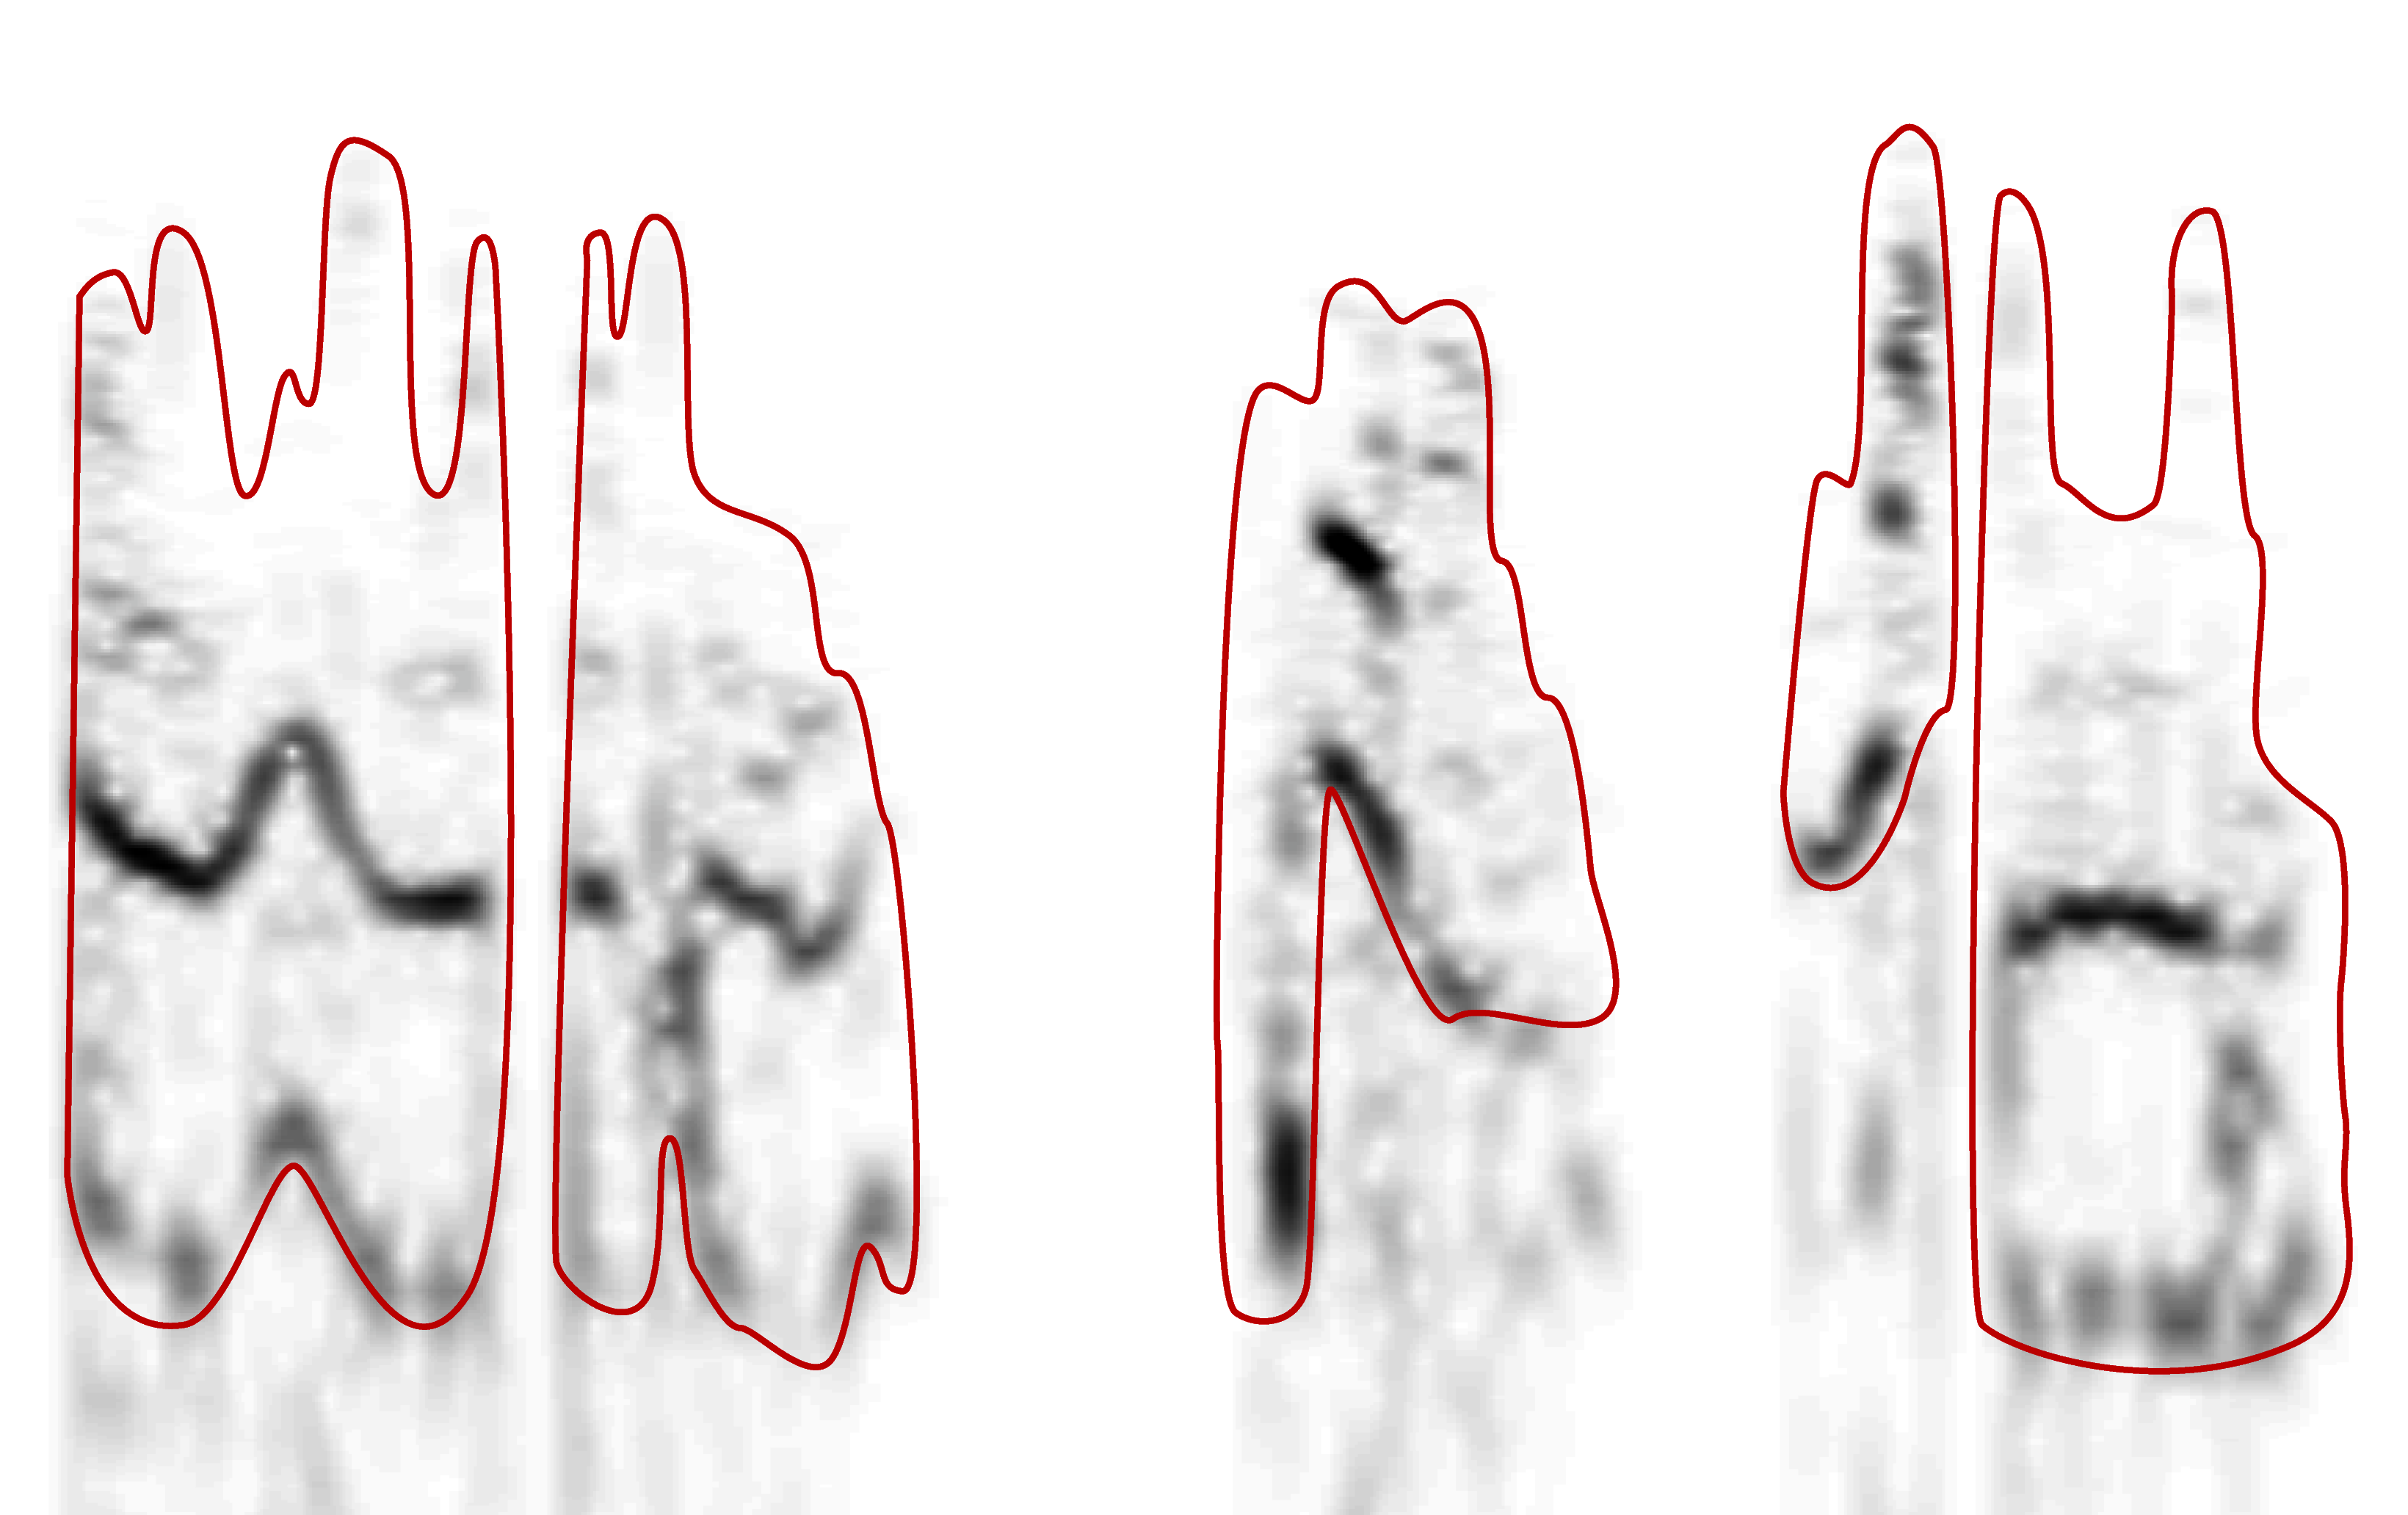
\includegraphics[width=10cm]{Chapter4/spectovocal.tif} %change centimeters for resizeing
   \caption{FFTFilter: Spectral mapping of vocal contour.}
   \label{fig:example}
\end{figure}
shows a spectrogram of speech and how the FFTFilter maps the contour of the vocal signal. Given that the vocal signal has a strong presence in a narrow frequency range, it is ideal to control the filter. FFTFilter therefore uses the continuos signal of the highest and lowest frequencies of the array to calculate the bandwidth and center frequency for the resonant filter. Figure 4.2 shows a visual representation of a fairly noisy signal that has been filtered by the resonant filter following the vocal contour as seen in Figure 4.1. 
\begin{figure}[htbp] %  figure placement: here, top, bottom, or page
   \centering
   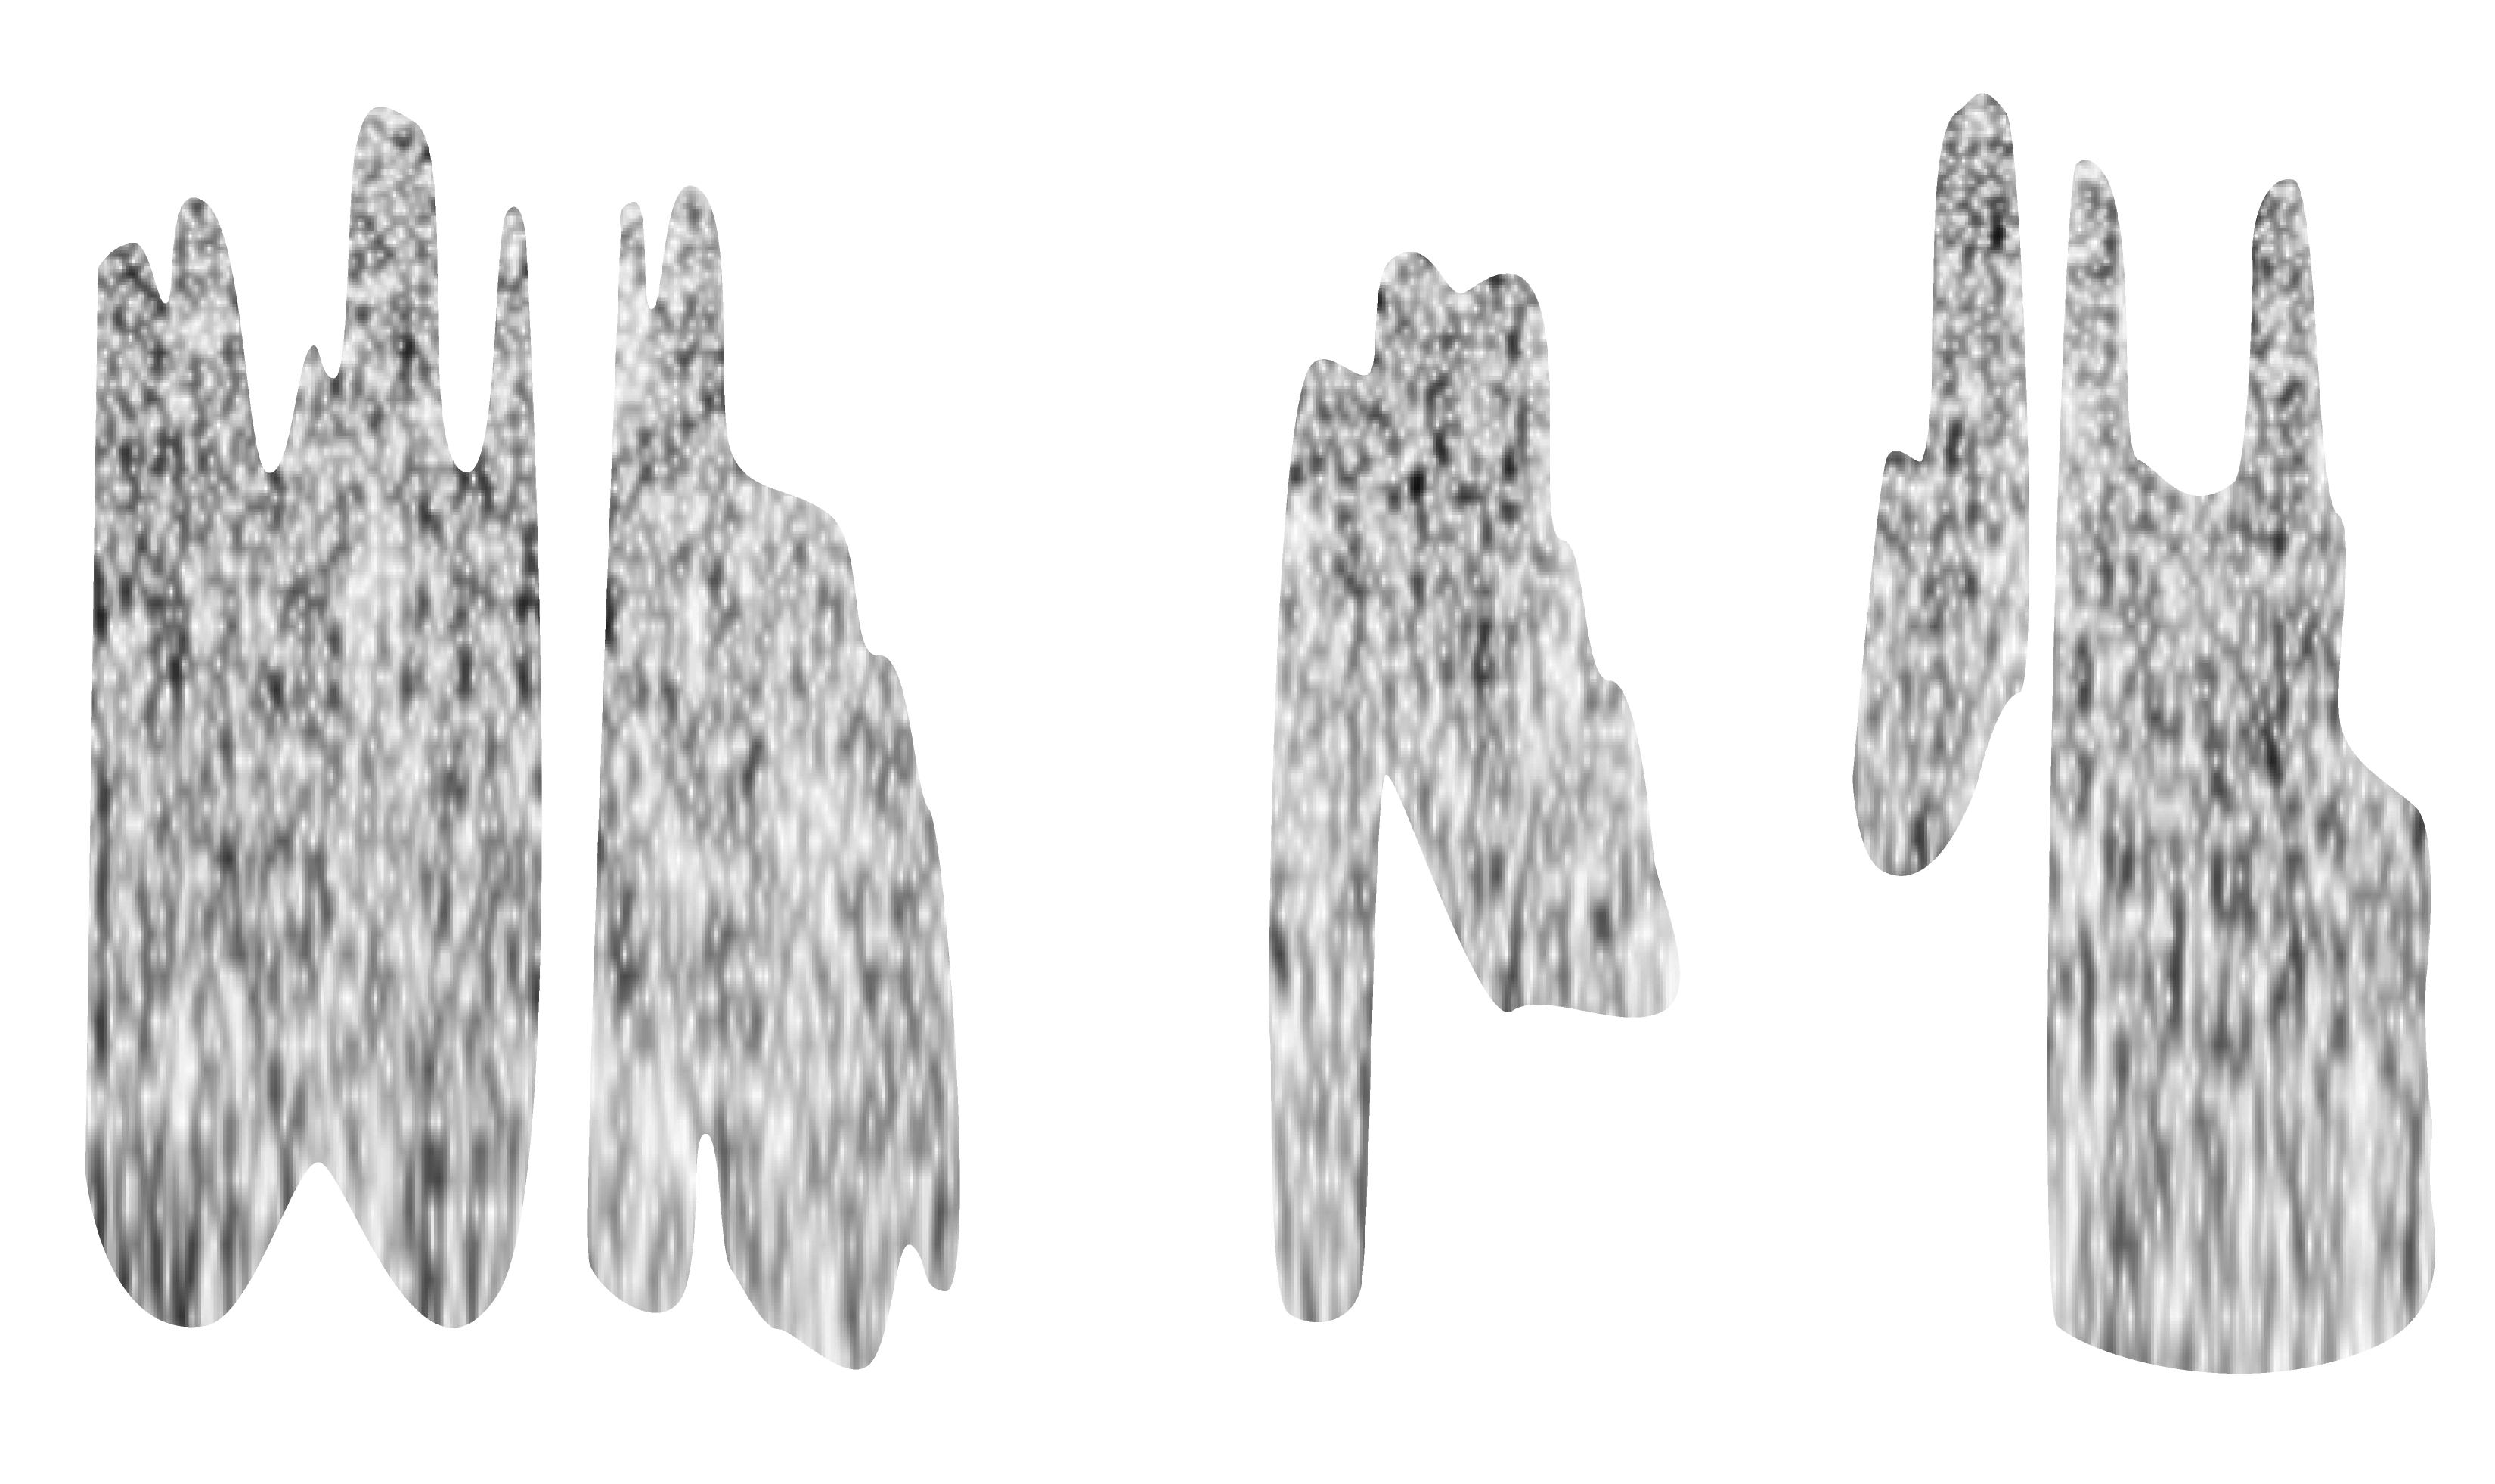
\includegraphics[width=10cm]{Chapter4/spectonoise.tif} %change centimeters for resizeing
   \caption{FFTFilter: Noise filtered by vocal contour.}
   \label{fig:example}
\end{figure}
Ones the trajectory of the filter is set by the frequency data extracted from the FFT, an envelope follower maps the amplitude of the sound that was used as the FFT input to control the amplitude of the resonant filter. By combining the amplitude envelope and frequency contour of one sound to control a resonant filter that is applied to another sound, it is possible to incorporate characteristics of the analyzed sound to the filtered sound source.

\subsection{SpearToSC and SpearToMIDI}

\href{http://github.com/freuben/FedeLib/blob/master/SpearToSC/SpearToSC.sc}{SpearToSC} is a class that takes data from the open source software application called SPEAR\footnote{Michael Klingbeil, SPEAR, 2005, URL: \href{http://www.klingbeil.com/spear/}{http://www.klingbeil.com/spear/}.} and transfers it to an array in SuperCollider. SPEAR uses a variation of the traditional McAulay-Quartieri procedure and ``attempts to represent a sound with many individual sinusoidal tracks (partials), each corresponding to a single sinusoidal wave with time varying frequency and amplitude.''\footnote{Michael Klingbeil, M. 2005. ``Software for spectral analysis, editing, and synthesis.'' in \emph{Proceedings of ICMC}, vol. 2005, 2005. URL: \href{http://www.klingbeil.com/papers/spearfinal05.pdf}{http://www.klingbeil.com/papers/spearfinal05.pdf}.} SPEAR provides a graphical representation of a sound\footnote{Spectral analysis, where the y-axis represents frequency in hertz and the x-axis represents time in seconds.} (as seen in Figure 4.3) in which it is possible to select the individual sinusoidal tracks and allows to isolate and access the information for each individual partial. 
\begin{figure}[htbp] %  figure placement: here, top, bottom, or page
   \centering
   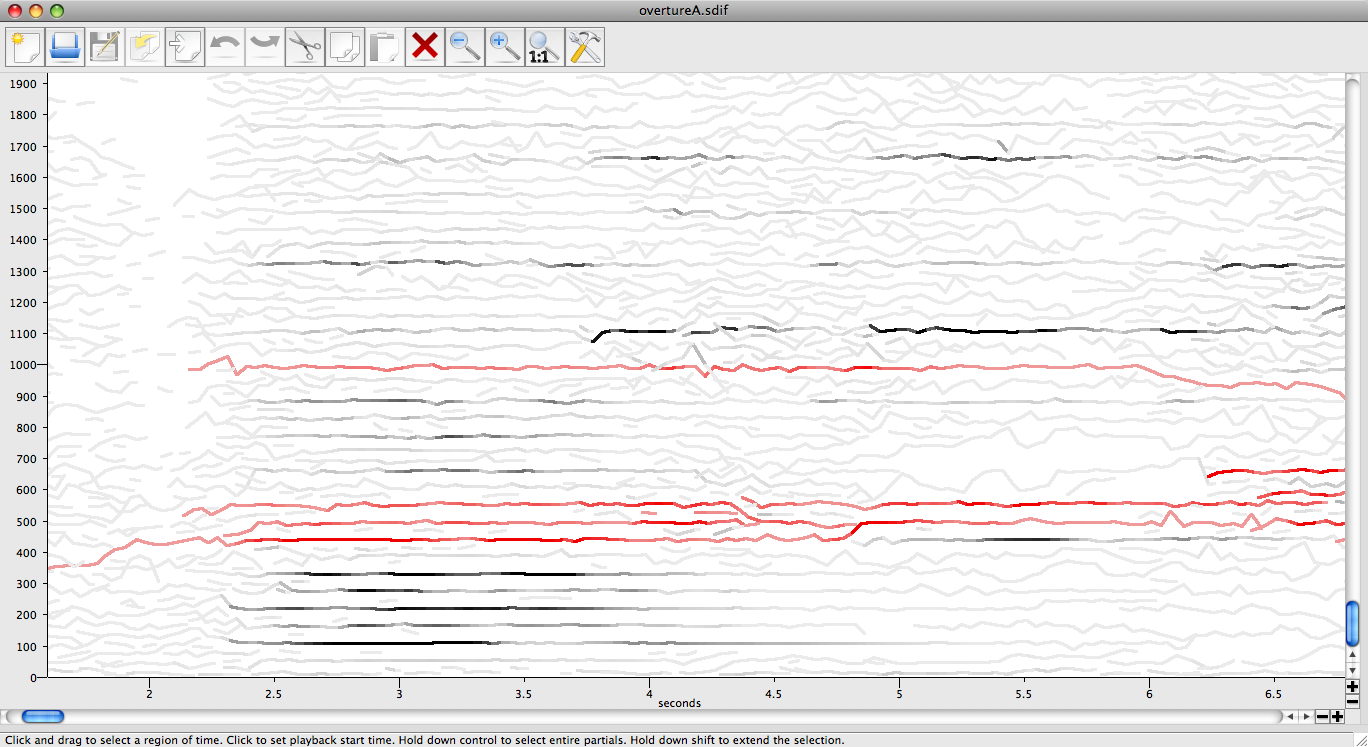
\includegraphics[width=15cm]{Chapter4/Spear1.tif} %change centimeters for resizeing
   \caption{SPEAR graphical interface.}
   \label{fig:example}
\end{figure}
The amplitude and frequency information of each partial is given by frame and can be stored in a text file. SpearToSC reads the text file produced by SPEAR\footnote{SpearToSC reads SPEAR text files in the \emph{Text - Partials} format only.} as a string and strips it into a multidimensional array in SuperCollider. It is therefore possible to access and manipulate this data within the SuperCollider language and server and re-synthesize this information not only with sinusoidal waves, but with any type of unit generator. 

\href{http://github.com/freuben/FedeLib/blob/master/SpearToSC/SpearToMIDI.sc}{SpearToMIDI} is a class that inherits functionality from SpearToSC and reduces the information given by SPEAR to be used as data to produce a MIDI file or to control SuperCollider synthesis definitions. The purpose of this class is to reduce the spectral information to an amount of data that can later produce notated material for a written score, a MIDI file or a control system to be used for triggering synthesis algorithms. The data in the text file generated by SPEAR is available by frame and gives too much information for this purpose. Therefore, SpearToMIDI reduces this data in four stages: First, it takes a magnitude threshold argument which gets rid of all of the partial information that lies bellow this value (as seen in Figure 4.4).
\begin{figure}[htbp] %  figure placement: here, top, bottom, or page
   \centering
   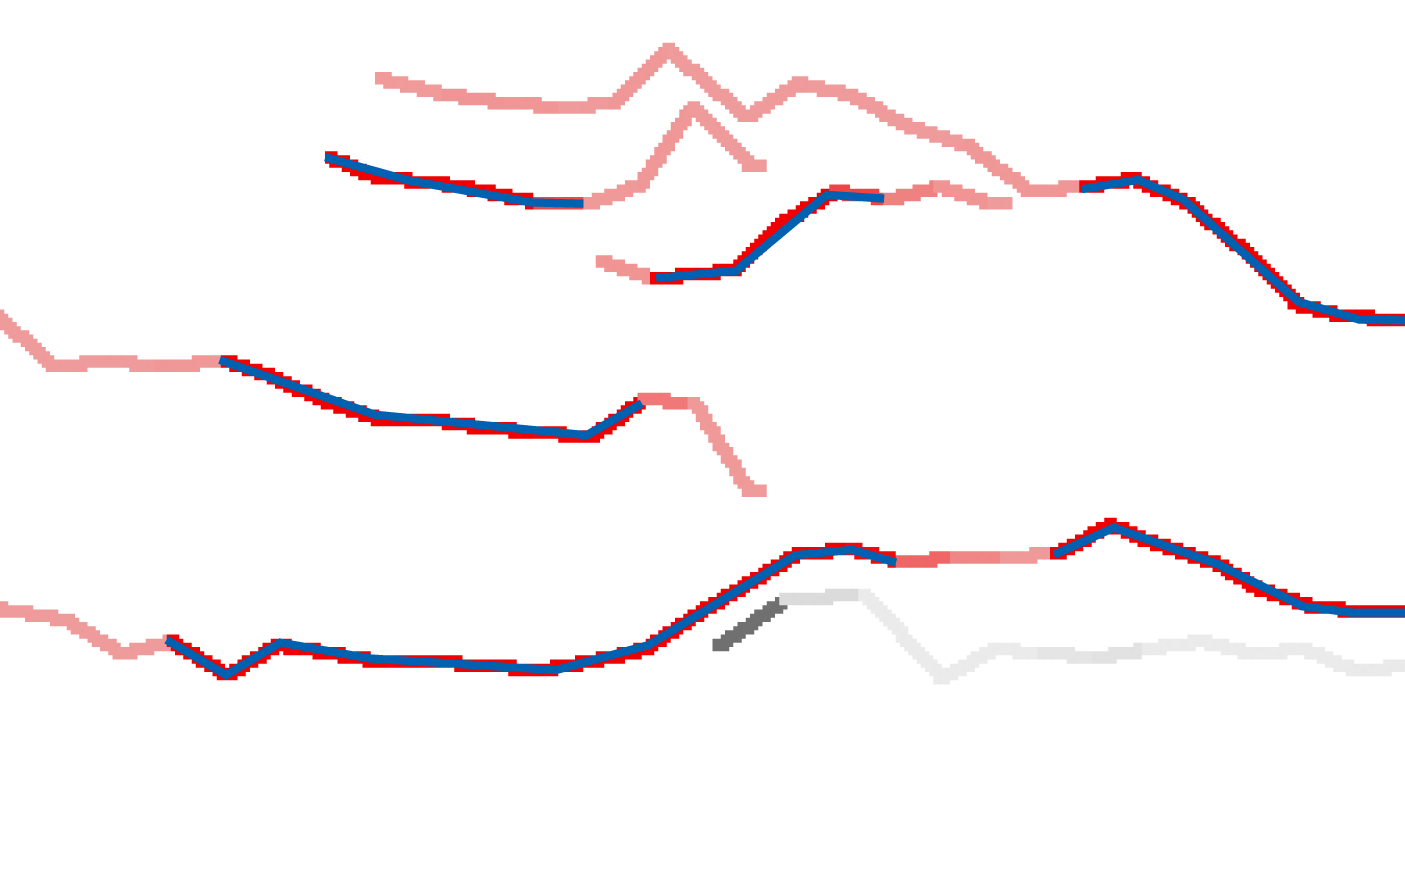
\includegraphics[width=9cm]{Chapter4/Spear2.tif} %change centimeters for resizeing
   \caption{SpearToMIDI: Amplitude threshold selection.}
   \label{fig:example}
\end{figure}\
In other words, it breaks the partial in different groups by introducing silences instead of the data that lies bellow the threshold and at the same time keeps track of the beginning and the end of each group. 

The second stage reduces data with a frequency modulation threshold. Each group is taken as a line and the computer only stores the points in the line which cross a given interval (the modulation threshold). For example, Figure 4.5 shows how the lines representing the groups in Figure 4.4 are traced by selecting the points that cross a given interval.\footnote{The grid represents the intervals as shown in the y-axis. For the purpose of simplification, the diagram doesn't show a logarithmic representation of frequency.} 
\begin{figure}[htbp] %  figure placement: here, top, bottom, or page
   \centering
   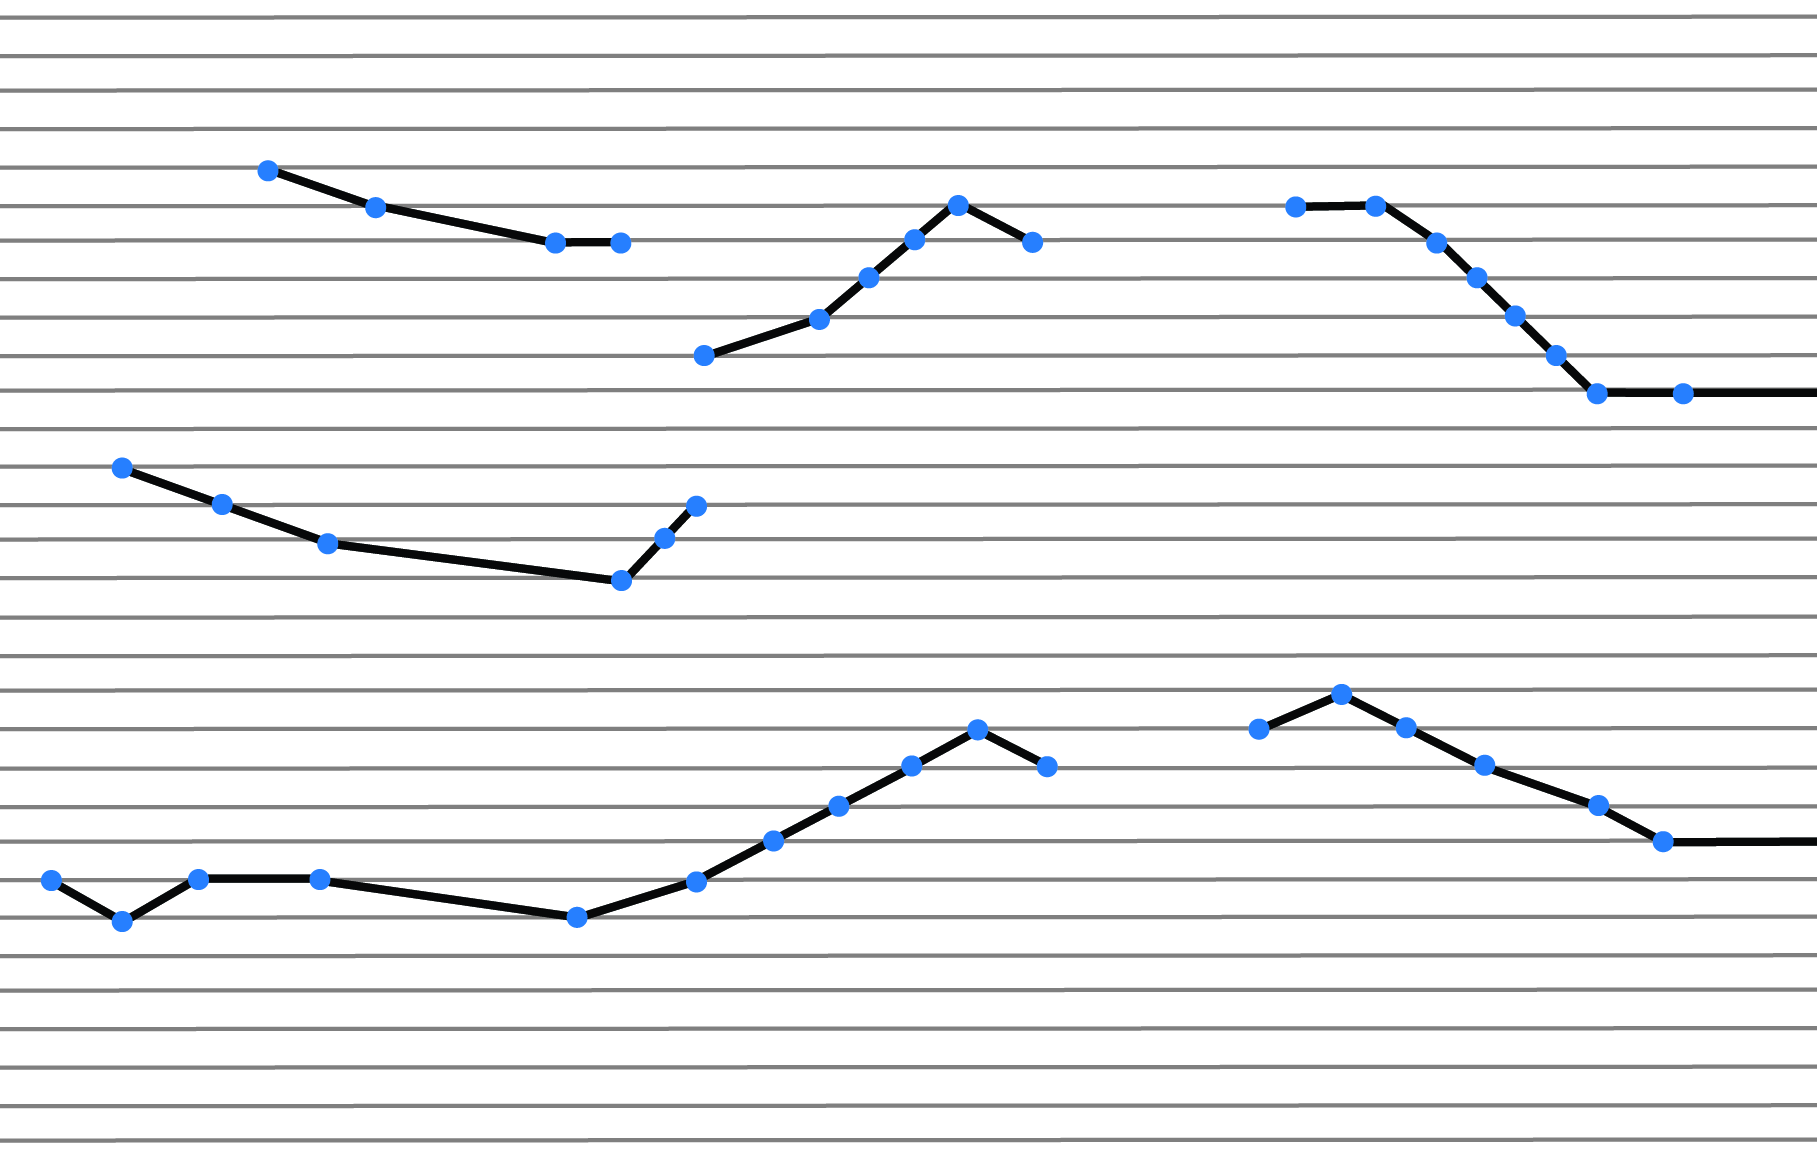
\includegraphics[width=10cm]{Chapter4/Spear3.tif} %change centimeters for resizeing
   \caption{SPEARToMIDI: Point selection through frequency modulation threshold.}
   \label{fig:example}
\end{figure}\
If the interval is of one semitone then the frequencies are averaged to the closest chromatic note. It is possible to make microtonal divisions of the equal-tempered scale by using floating point values for the modulation threshold. The magnitude, frequency and time values of each point are stored as a collection of data. This collection can then be accessed and used to control synthesis definitions externally by generating envelopes, which gradually change frequency to produce glissandos and amplitude for gradual volume change. After these first two stages, the original data from Spear is reduced considerably by disregarding details that are not vital for the given purpose. 

The third stage, takes the points of the lines that were obtained in the previous stage and translates them into single notes with a start and an end and that do not change in frequency and amplitude while playing--- in other words, a format that is compatible with the MIDI note-on and note-off paradigm. The points are then considered as representing note-on messages and the note-off messages are calculated depending on whether the point is followed by another new point or if the point is the last of the group, in which case a silence would proceed. In other words, a note-off is inserted before a new note-on or just before a silence. Figure 4.7 
\begin{figure}[htbp] %  figure placement: here, top, bottom, or page
   \centering
   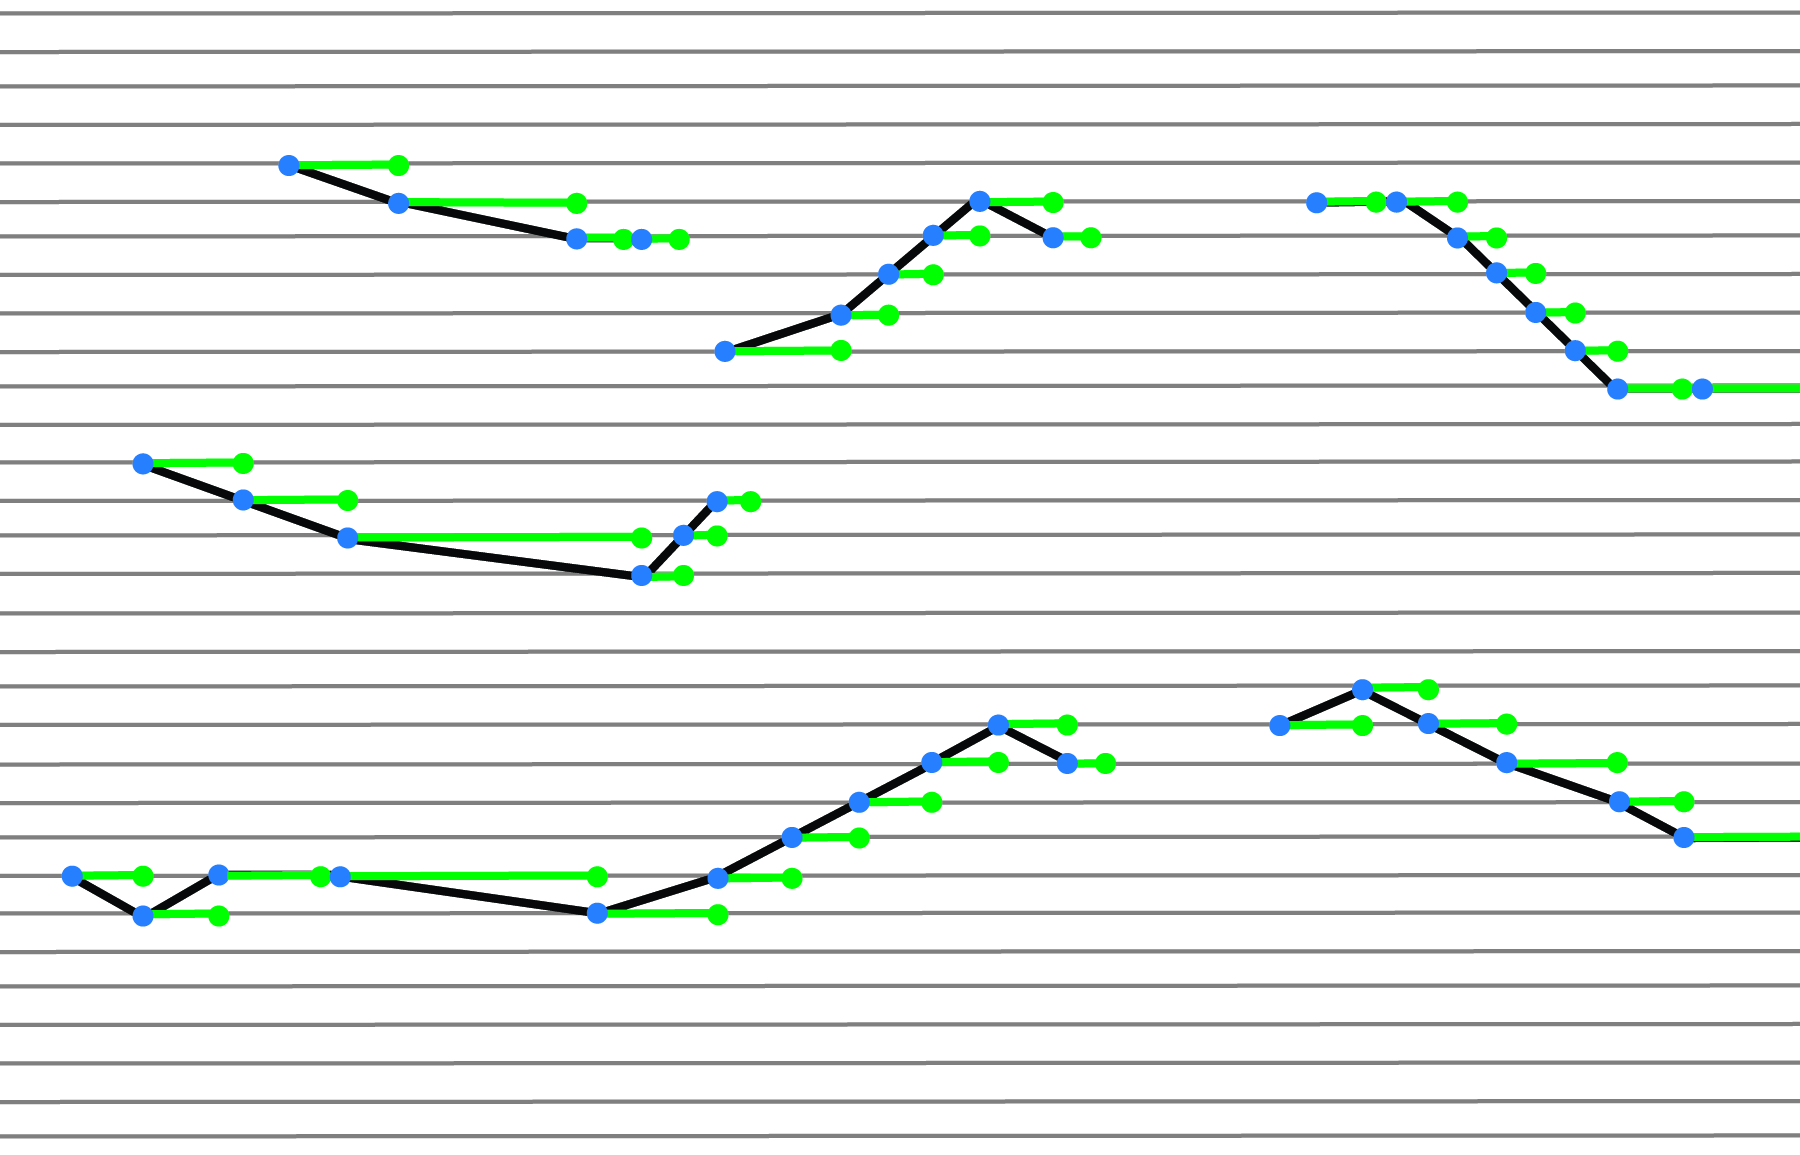
\includegraphics[width=10cm]{Chapter4/Spear4.tif} %change centimeters for resizeing
   \caption{SPEARToMIDI: Note representation.}
   \label{fig:example}
\end{figure}\
shows the note representation derived from Figure 4.5, where the notes are seen as green lines, the note-on messages as blue points and the note off messages as green points. 
The results of this stage can be used to generate a MIDI file\footnote{Using the SimpleMIDIFile class that is part of wslib by \href{http://www.woutersnoei.nl/}{Wouter Snoei}, which is can be obtained as a Quark.} with the intention of either using it to trigger a sampler or to import it into a notation software to create a written score. The user can input the time signature and tempo for the MIDI file as well as an interval value that divides the MIDI note range into different MIDI tracks. By doing this, the notes are separated into different tracks depending on their value in relationship to each other with the purpose of not having too many notes in the same track. Furthermore, these results can be used to create a list of Open Sound Control (OSC)\footnote{See \href{http://opensoundcontrol.org/introduction-osc}{http://opensoundcontrol.org/introduction-osc} for more information on OSC.} commands that can be sent to the SuperCollider server for Real-Time-Synthesis and Non-Real-Time-Synthesis. Extra arguments can also be added to control other values in the synthesis definition, which can be set individually by using a function to be evaluated for each instance of the definition.

\section{Real-Time Scoring}

\emph{Interpassivity.} Improvisation, etc.
Display as score. Score animations...

\subsection{AlgorithmicScore}

\href{http://github.com/freuben/FedeLib/blob/master/AlgorithmicScore/AlgorithmicScore.sc}{AlgorithmicScore} is a class that visualizes different types of notation in real-time. It is programmed as a graphical user interface (GUI) in SuperCollider but receives no input in the GUI window itself. Instead, this class only displays notes, letters, symbols and other visual aids for real-time scoring from code that can be evaluated in the interpreter, or within a compiled class in the SuperCollider language. It displays some traditional musical symbols including notes, accidentals, clefs, dynamics, etc., that are readymade fonts in combination with non-standard notations. Stems and flags are purposely not implemented to not give too much visual information to the performer while following the score. Note-heads can be of different type and color. There are four types of different clefs that are implemented: treble, bass, alto, tenor.  If a clef is selected, a staff is generated in which the notes will appear. The information to be placed in the score can be evaluated in an array consisting of the note position from left to right, staff number, note-head type, note, accidental and color. There are three array types that can be used which respond to different notation modes: free, enharmonic and chromatic. In the free mode, notes are selected by a number that does not correspond to the clef but to the position from top to bottom starting with zero as the first leisure line bellow the bottom line of the staff. Moreover, the note value can not only be negative but also a float number, which results in a position in between notes. This mode can be useful for conveying movement if the score were to be animated. The enharmonic mode, takes a string representing the note and octave---were c4 equals middle C---and positions the note according to the selected clef. It is also possible to select the type of accidental between flat, sharp and natural. Additionally, if the note exceeds four leisure lines, the programme places an \emph{8va} sign and if it is an octave bellow that, it places a \emph{15ma} sign. The chromatic mode, is similar to the enharmonic, but only uses sharps as accidentals and places a natural in front of each note that is diatonic. This mode is useful to receive note information as midi numbers.

The following piece of code, generates a new window and 

\begin{verbatim}
a = AlgorithmicScore.screenBounds;
a.score([\bass, \treble, \treble], 1.0, 1, 1.3);
//[pos, [staff, noteType, note, acc, color]]:
~staff1 = [[0, [0, 1, "c3"]], [1, [0, 0, "b3", \flat, \blue]]]; 
~staff2 = [[0, [1, 0, "d5", \flat]]];
~staff3 = [[0, [2, 1, "a3", \nat, \red]]];
a.enharmonic(~staff1 ++ ~staff2 ++ ~staff3); //writes notes
a.expression("p"); //expression for dynamics
a.text("Improvise with pitch material", "Helvetica", 30, 30, 200, 1, Color.rand);
\end{verbatim}

The result:

\begin{figure}[htbp] %  figure placement: here, top, bottom, or page
   \centering
   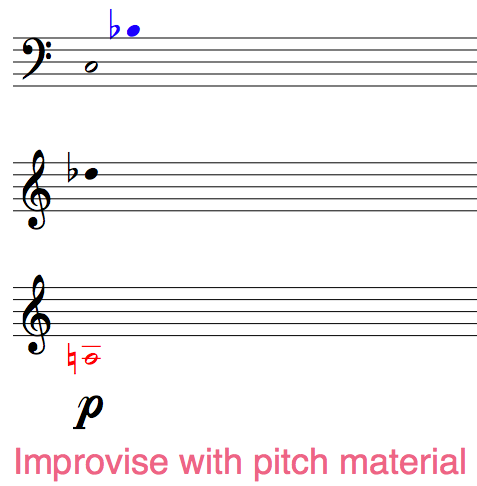
\includegraphics[width=10cm]{Chapter4/algoscore1.tif} %change centimeters for resizeing
   \caption{AlgorithmicScore: Enharmonic mode.}
   \label{fig:example}
\end{figure}\


\begin{figure}[htbp] %  figure placement: here, top, bottom, or page
   \centering
   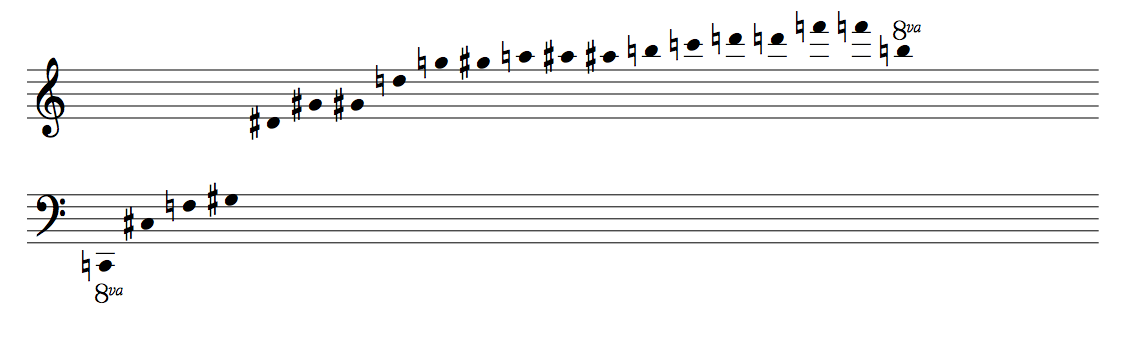
\includegraphics[width=17cm]{Chapter4/algoScore_partials.tif} %change centimeters for resizeing
   \caption{AlgorithmicScore: PartialTracker to Notes.}
   \label{fig:example}
\end{figure}\

\section{Pre-compositional Tools}

\subsection{MIDI Mapping}

\subsection{MIDI Triggering}

\label{ch:compamp}